虽然吲哚骨架在自然界中是普遍存在的,但是在苯环的任意位置上又加了个环的吲哚却并不常见。Trikentrins和结构相似的herbindoles代表了6,7-增环的吲哚或多烷基化的环戊烯基{[}g{]}吲哚天然产物。从蜘蛛海绵内分离出来的Trikentrin具有抗菌活性。下图展示了Trikentrin
A的可能结构。在此问题中,我们将找出以下结构中哪个是Trikentrin A。

\begin{figure}[h]
	\centering
	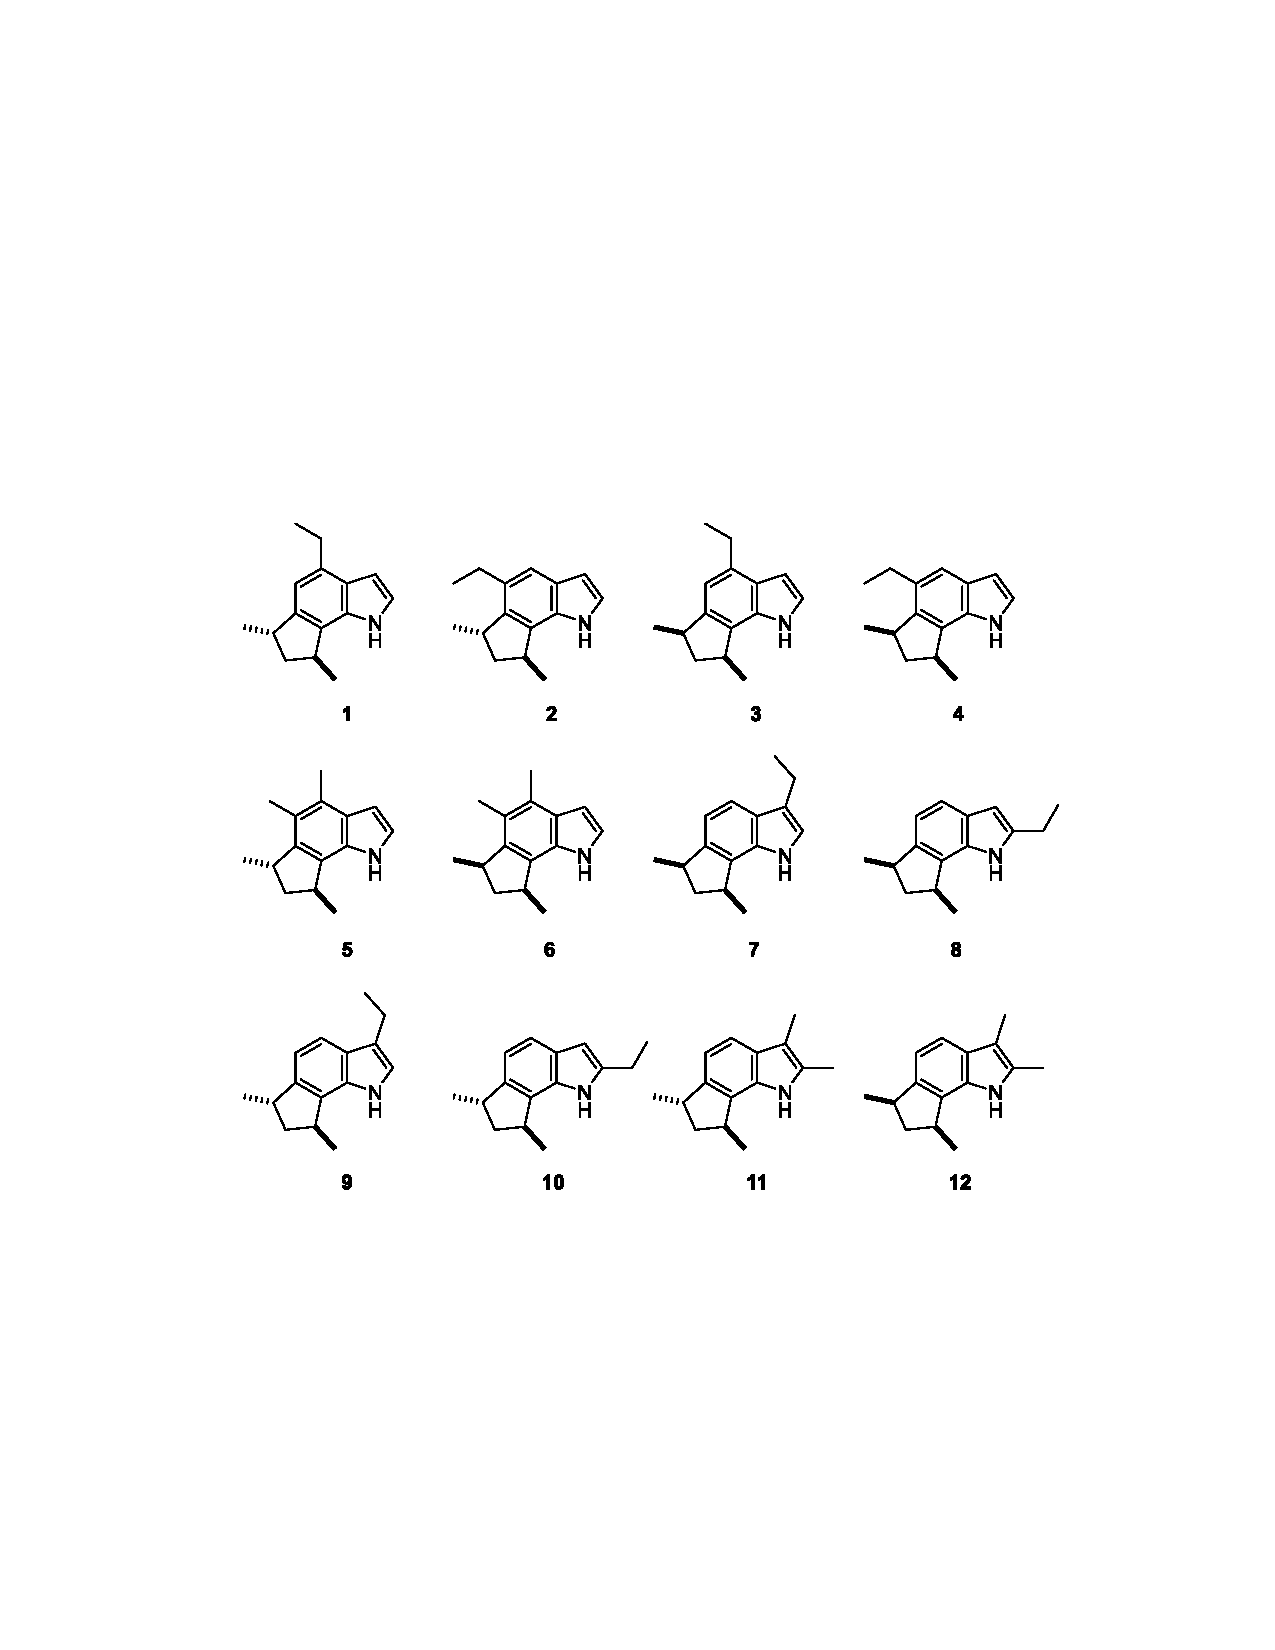
\includegraphics[width=14cm]{./pic/t7-1.pdf}
\end{figure}

合成Trikentrin
A的方法有几种:下面的两条路线包括基于芳炔的策略以及氢化乙烯基化的策略。试题7.1与7.2中的第一步是Bartoli吲哚合成法,即邻取代硝基芳香化合物与乙烯基格式试剂反应生成取代吲哚的反应。特别的,这也是合成7-取代吲哚的最有效的途径。

\begin{figure}[h]
	\centering
	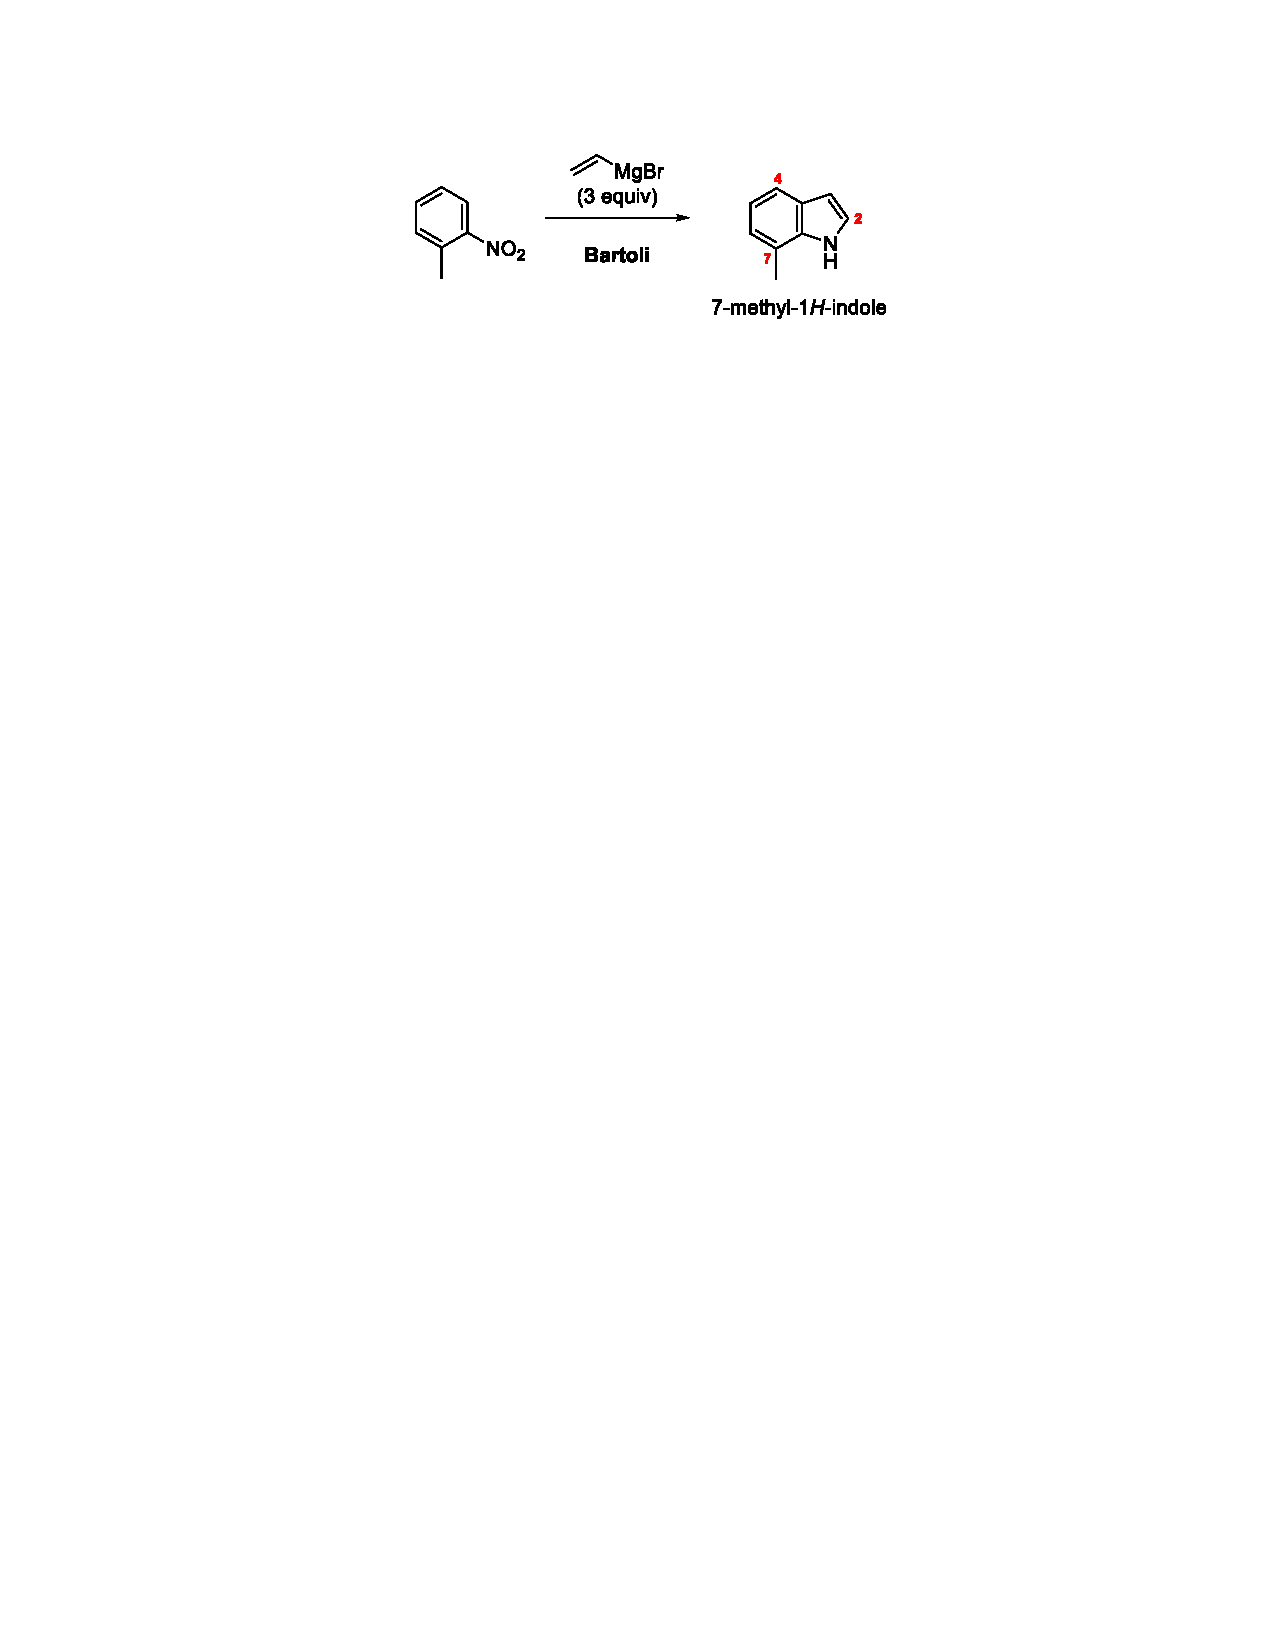
\includegraphics[width=9cm]{./pic/t7-2.pdf}
\end{figure}

\noindent(±)-Trikentrin A\textbf{:} \textsuperscript{1}H NMR
(CDCl\textsubscript{3}): $\delta$ 8.08 (bs, NH, 1H), 7.15−6.59 (3H), 3.44 (dt, \emph{J} = 8.8, 7.5 Hz, 1H), 3.22 (dt, \emph{J} = 8.8, 7.5 Hz, 1H), 2.94 (dq, \emph{J} = 15.0, 7.5 Hz, 1H), 2.93 (dq, \emph{J} = 15.0, 7.5 Hz, 1H), 2.60 (dt, \emph{J} = 12.3, 7.5 Hz, 1H), 1.50 (d, \emph{J} = 6.8 Hz, 3H), 1.37 (d, \emph{J} = 7.0 Hz, 3H), 1.36 (t, \emph{J} = 7.5 Hz, 3H), 1.32 (dt, \emph{J} = 12.3, 8.8 Hz, 1H); \textsuperscript{13}C NMR (CDCl\textsubscript{3}): $\delta$ 143.4−101.6 (8 signals), 44.8−15.1 (7 signals).

\newpage\noindent\textbf{基于芳炔的策略}

\begin{figure}[h]
	\centering
	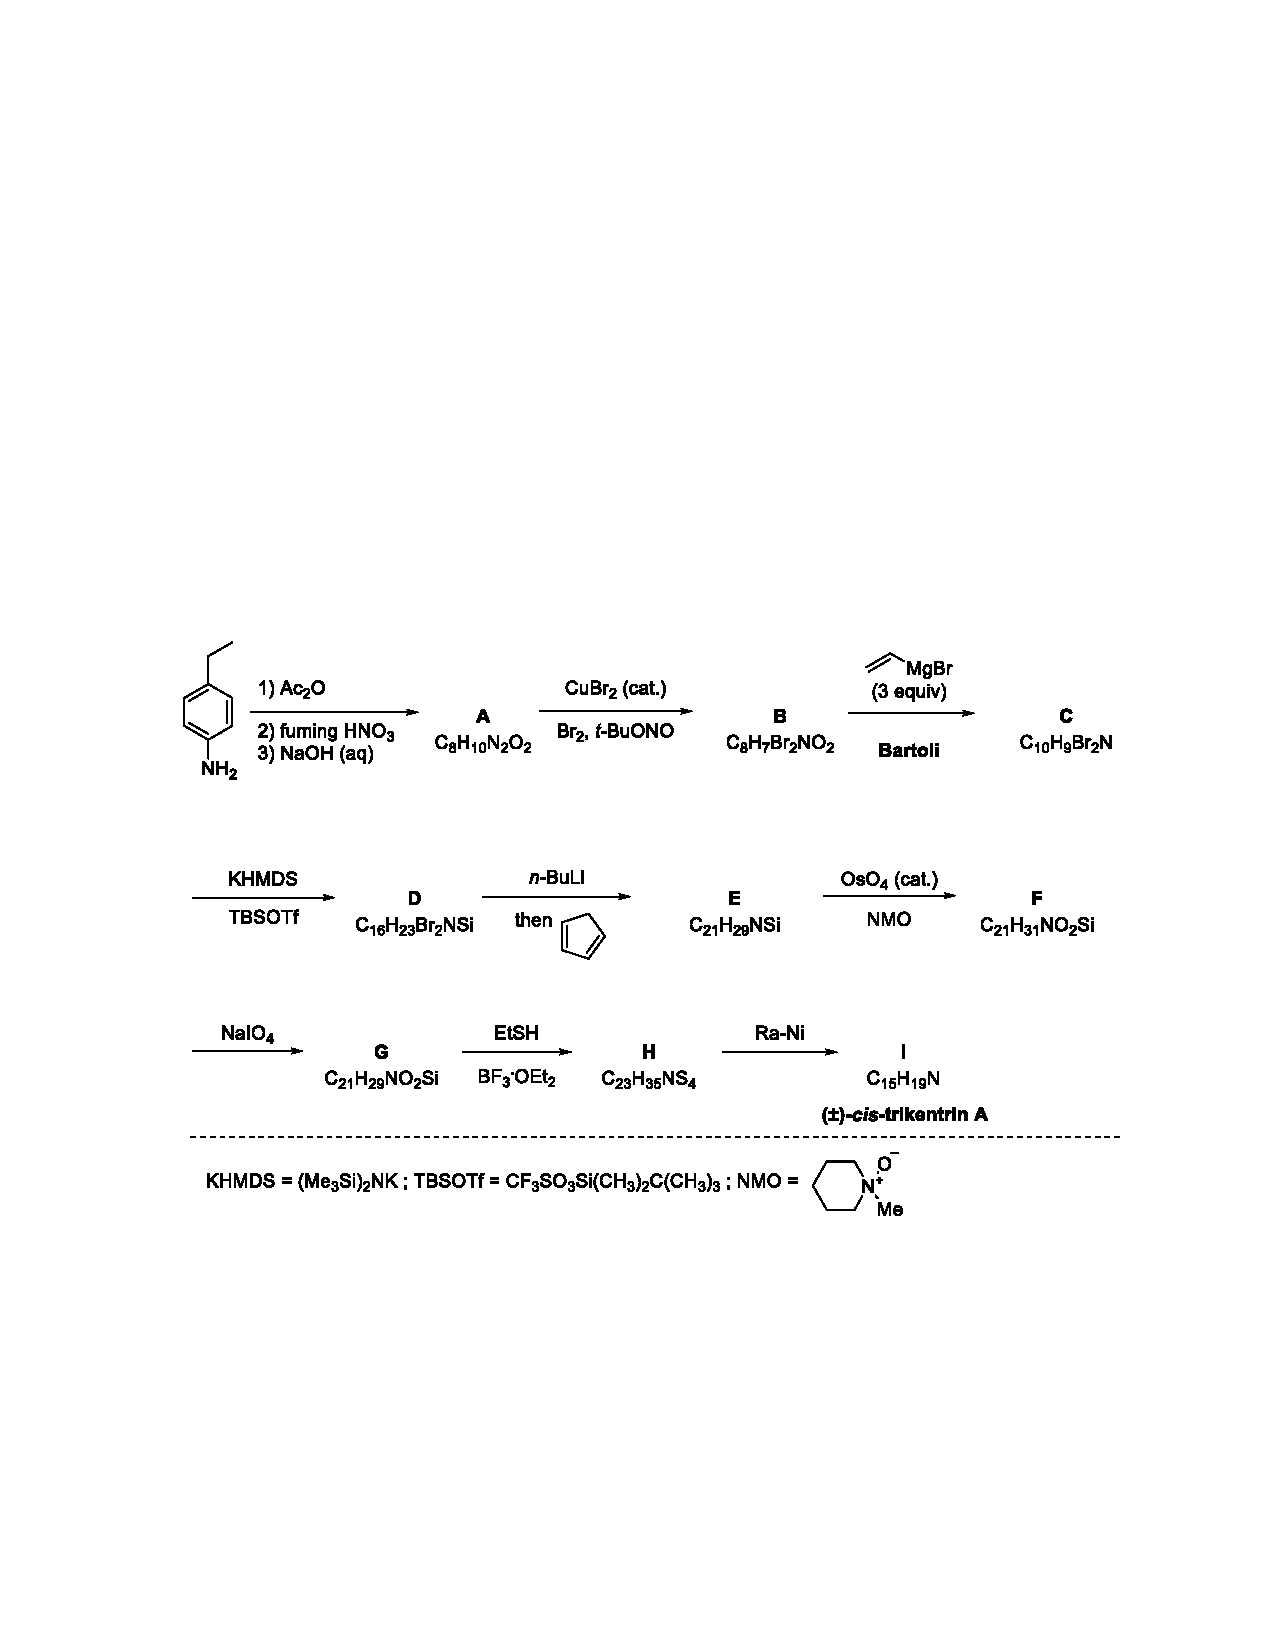
\includegraphics[width=16cm]{./pic/t7-3.pdf}
\end{figure}

\noindent\textbf{7.1.} 画出\textbf{A}-\textbf{I}的结构。

\noindent\textbf{7.2.} 画出步骤\textbf{D}-\textbf{E}中芳炔中间体的结构。

\noindent\textbf{氢化乙烯基化策略}

\begin{figure}[h!]
	\centering
	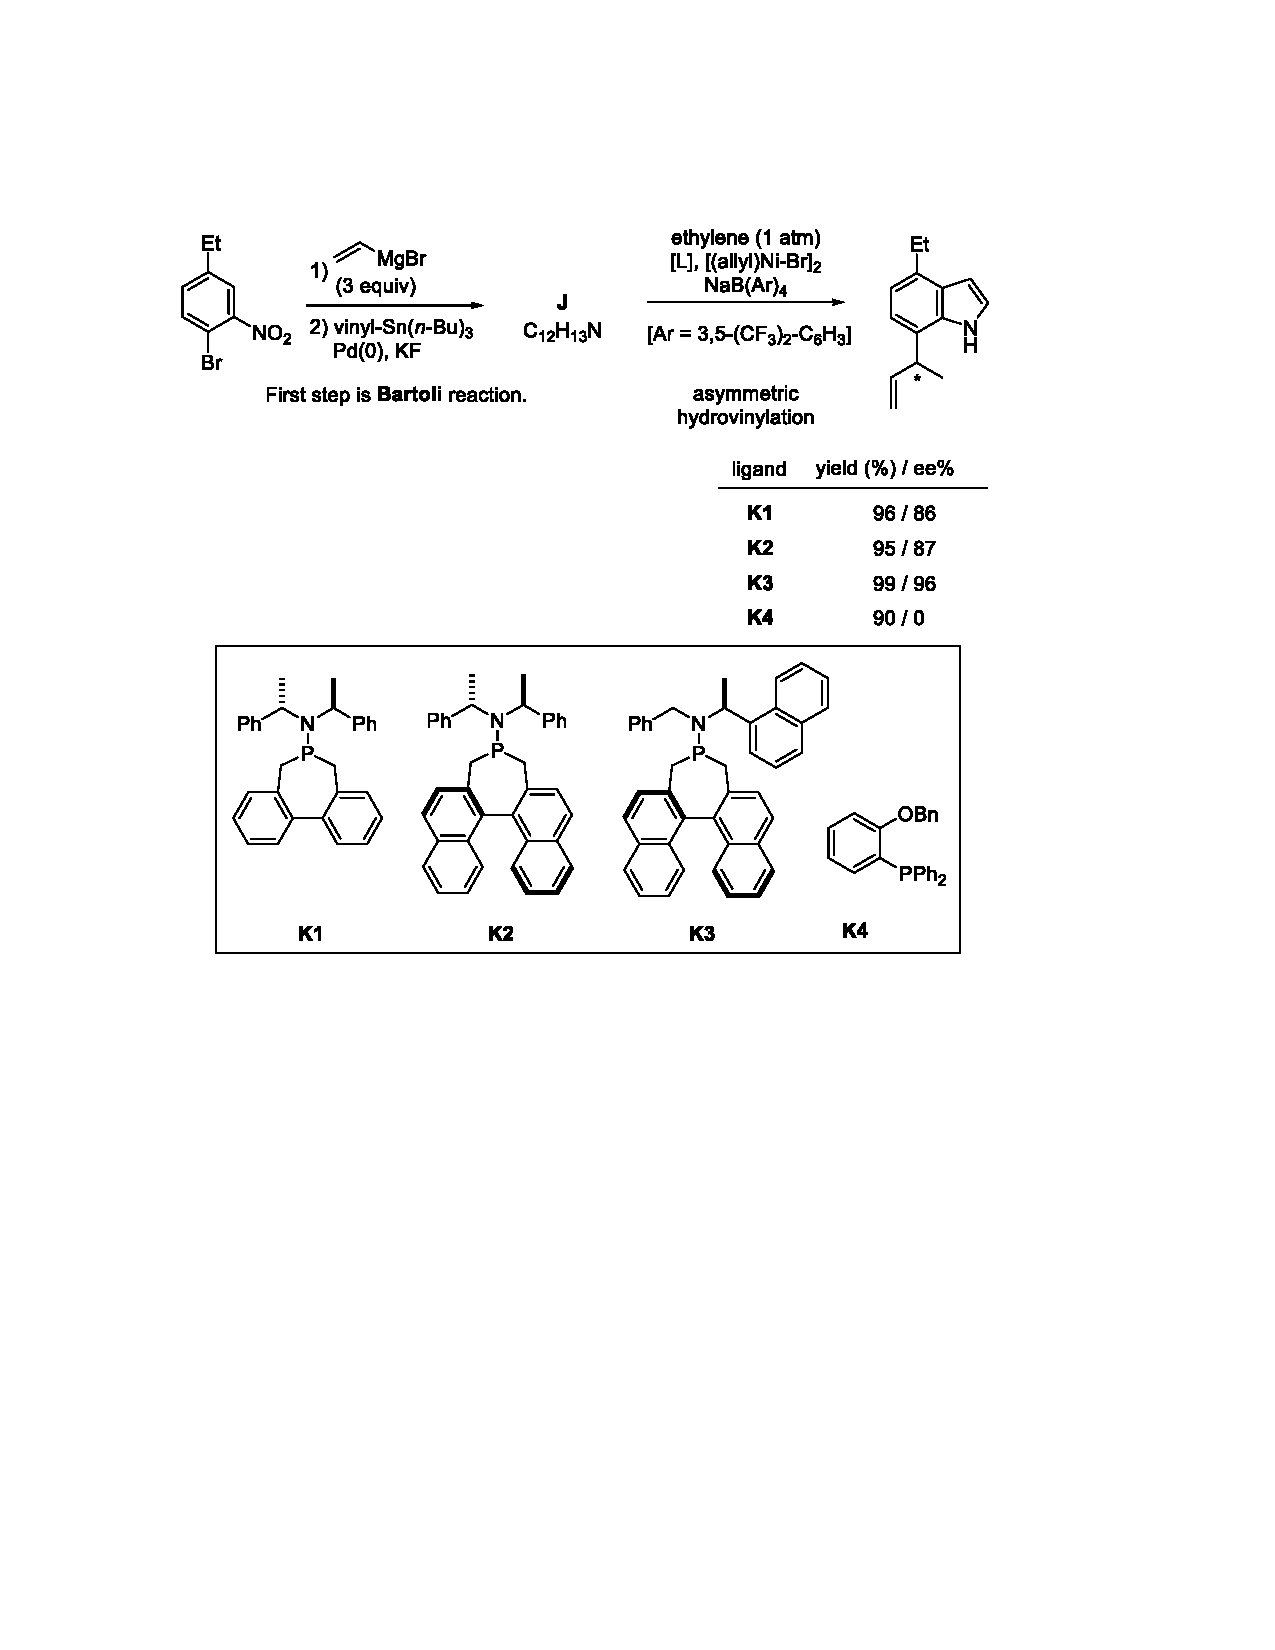
\includegraphics[width=14cm]{./pic/t7-4.pdf}
\end{figure}

\noindent\textbf{7.3.}
从溴代硝基苯到对应的7-乙烯基吲哚\textbf{J}的转化包括了Bartoli吲哚合成法及随后使用乙烯基锡的乙烯基化。画出\textbf{J}的结构。

第二步是Ni(II)催化的不对称氢化乙烯基化反应。该反应的配体\textbf{K1}-\textbf{K4}已在上图给出。

\noindent 注:ee为对映体过量,ee\%=占多数的对映体百分含量-占少数的对映体百分含量

\noindent\textbf{7.4.} 判断以下陈述:

\renewcommand{\labelitemi}{$\square$}
\begin{itemize}
\item 配体\textbf{3}给出了最好的对映体选择性
\item 配体\textbf{4}给出了外消旋体
\item 以上四个配体都是具有手性的
\item 以上四个配体都给出了很高的产率(\textgreater{}95\%)
\end{itemize}
\renewcommand{\labelitemi}{$\bullet$}

\noindent\textbf{7.5.} 对于氢化乙烯基化一步,判断以下陈述:

\renewcommand{\labelitemi}{$\square$}
\begin{itemize}
\item 烯丙基溴化镍是乙烯基的来源。
\item 在此烯丙基镍配合物中,镍的氧化态为+2。
\item 在此烯丙基镍配合物中,镍的外层电子数为18。
\item 此镍配合物具有平面四方的立体构型。
\end{itemize}
\renewcommand{\labelitemi}{$\bullet$}

\begin{figure}[h!]
	\centering
	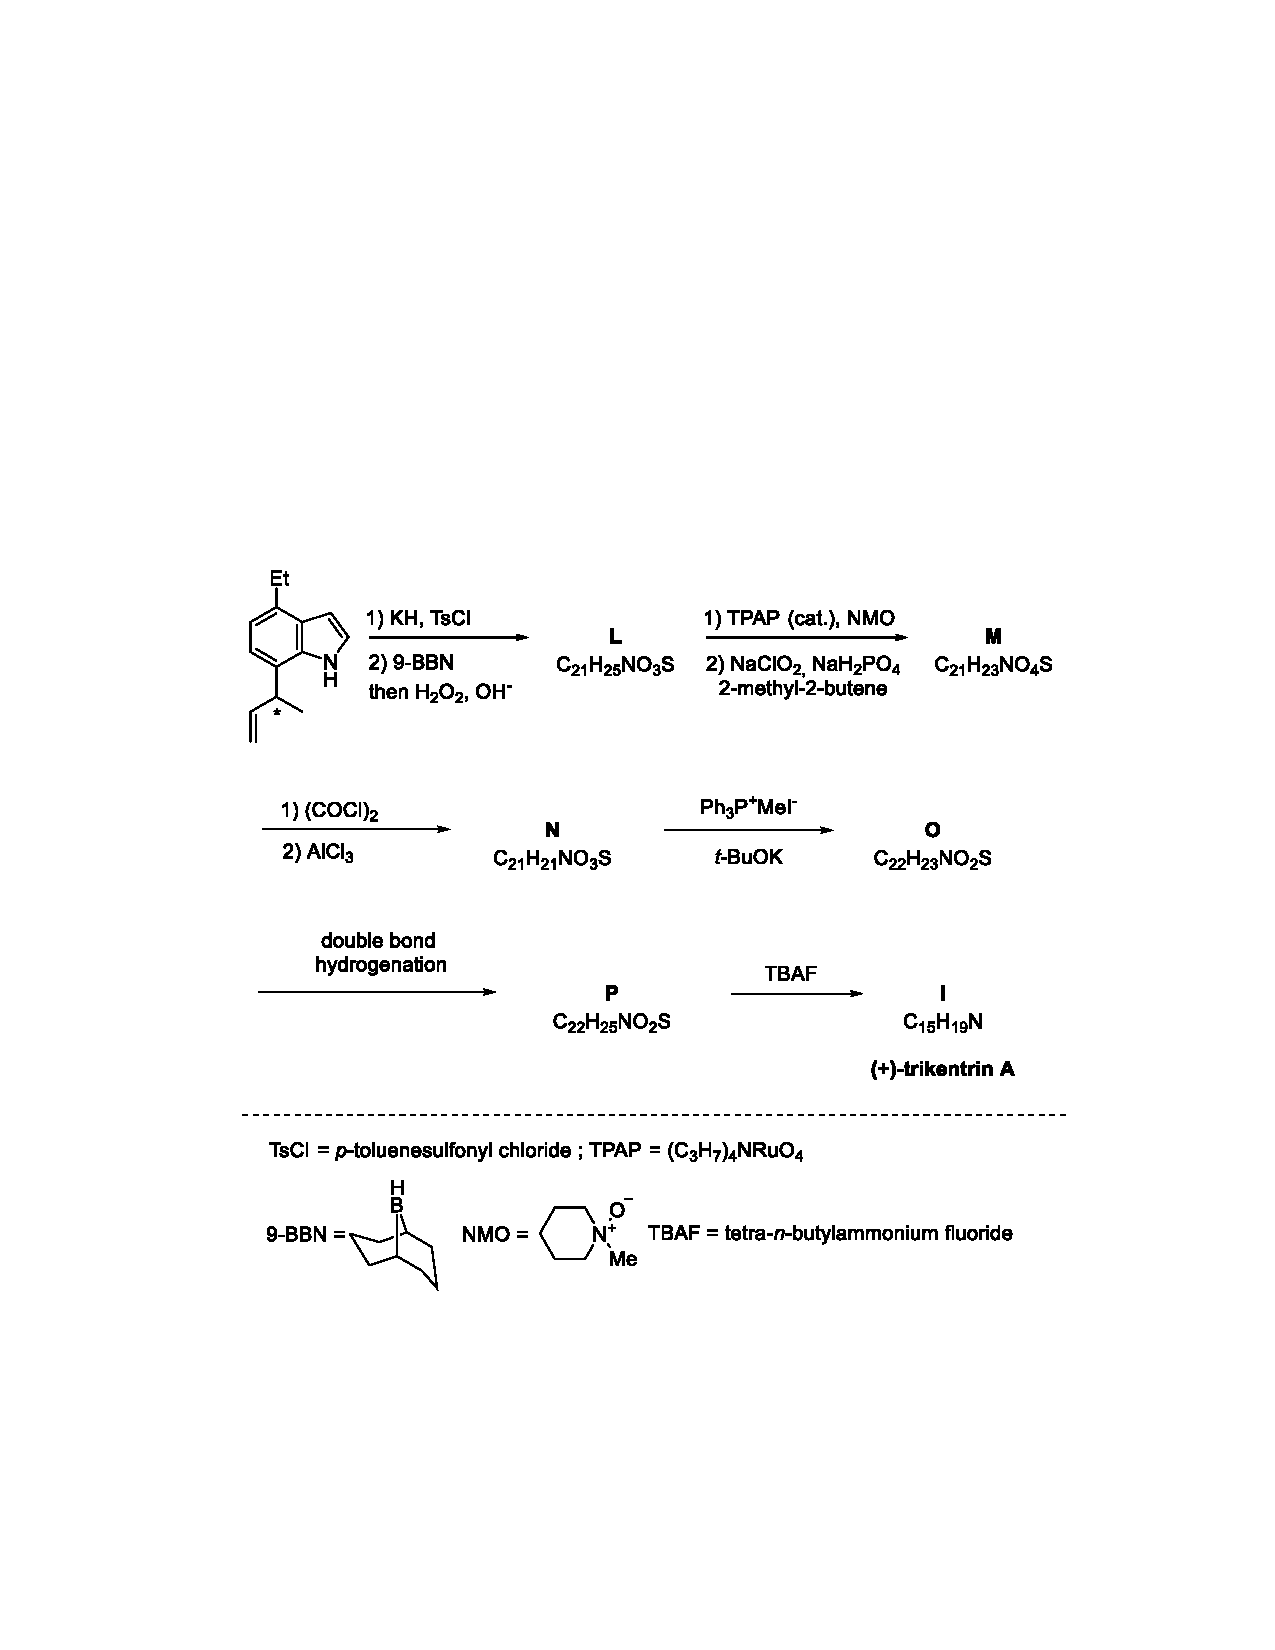
\includegraphics[width=14cm]{./pic/t7-5.pdf}
\end{figure}

\noindent\textbf{7.6.}
画出\textbf{L-P}的结构。氢化乙烯基化的产物之绝对构型为S。提示:在化合物\textbf{M}的\textsuperscript{13}C
NMR谱中,有一个峰在$\delta$ = 178.33 ppm处被观测到。


\textbf{\\
}
